%Florian Bogner
%e1225415
%Optimierung der Anzahl der Ausbildungstellen im österreichischen Gesundheitssystem
%Bacc-Seminar

\documentclass[a4paper,12pt]{article}
\usepackage{fullpage}
\usepackage[utf8]{inputenc}
\usepackage[ngerman]{babel}
\usepackage{amsmath}
\usepackage{amssymb}
\usepackage{latexsym}
\usepackage{mathtools}
\usepackage{listings}
\usepackage{algorithm}
\usepackage{algpseudocode}
\usepackage{graphicx}
\usepackage{booktabs}
\usepackage{hhline}

\begin{document}

\begin{titlepage}
\huge
\centering
Optimierung der Anzahl der Ausbildungstellen im österreichischen Gesundheitssystem 

\vfill

\normalsize
Florian Bogner

Betreut von: Claire Rippinger \& Christoph Urach
%oder whs der Breitenegger
\end{titlepage}




\tableofcontents
\newpage

\section{Abstract}

We attempt to calibrate a model of the austrian healthcare system. Our goal is to make sure retiring doctors are replaced by freshmen in equal numbers. To achive this we test three algorithms, namly Particle Swarm, Great Deluge and Downhill Simplex Optimization. We identify a function to judge model outputs and optimize based on that. Experiments show that the Particle Swarm is the best of out approaches with Downhill Simplex as close second. Great Deluge instead fails to yield satisfing results.

\section{Einleitung}

In dem von $dexhelpp$ geschaffenen Modell für die Laufbahn österreichischer Ärzte von Studienbeginn bis Pensionierung sollen bestimmte Parameter via Optimierungsalgorithmen kalibriert werden. Da das Modell sehr detailliert und komplex ist, dauert ein Simulationsdurchlauf mehrere Minuten. Deshalb ist es notwendig Algorithmen zu finden, die mit Simulationsauswertungen sehr sparsam umgehen. 

\subsection{Das Modell}

Es handelt sich um ein agentenbasiertes Modell. Die Agenten repräsentieren ÄrztInnen an verschiedenen Stellen in ihrer Ausbildung oder ihrem Berufsleben. Sie beginnen als Studenten an einer der sieben Universitäten für Medizin in Österreich. Nach dem Studienabschluss beginnen die Agenten mit ihrem Turnus, entweder als Allgemeinmediziner (AM) oder Facharzt (FA). Absolventen der AM-Ausbildung entscheiden sich dann ob sie als AM berufstätig werden oder die FA-Ausbildung beginnen. 

Die Ausbildung im Turnus und das Berufsleben ist aufgeteilt auf die neun Bundesländer und weiter aufgeteilt auf den Urbanisationsgrad (Städte, Kleinstädte und Vororte, Ländliche Gebiete). Die Agenten treffen während ihrer Laufbahn viele Entscheidungen wie z.B. Studienwechsel, Emigration, Wahl der Ausbildungsstelle, Berufswechsel, Vollzeit oder Teilzeit, etc. 

Das ganze Modell hat hunderte Parameter, die zum größten Teil aus Expertenschätzungen bestehen oder aus historischen Daten extrapoliert wurden. Der Anfangszustand besteht aus aktuellen echten Daten. Das Modell wird dann bis zu einem festgelegtem Jahr durchgerechnet und Informationen über alle Agenten in Form einer Datenbank gespeichert. Aus dieser kann man dann alles auslesen, was man beobachten will.

\begin{figure}[h]
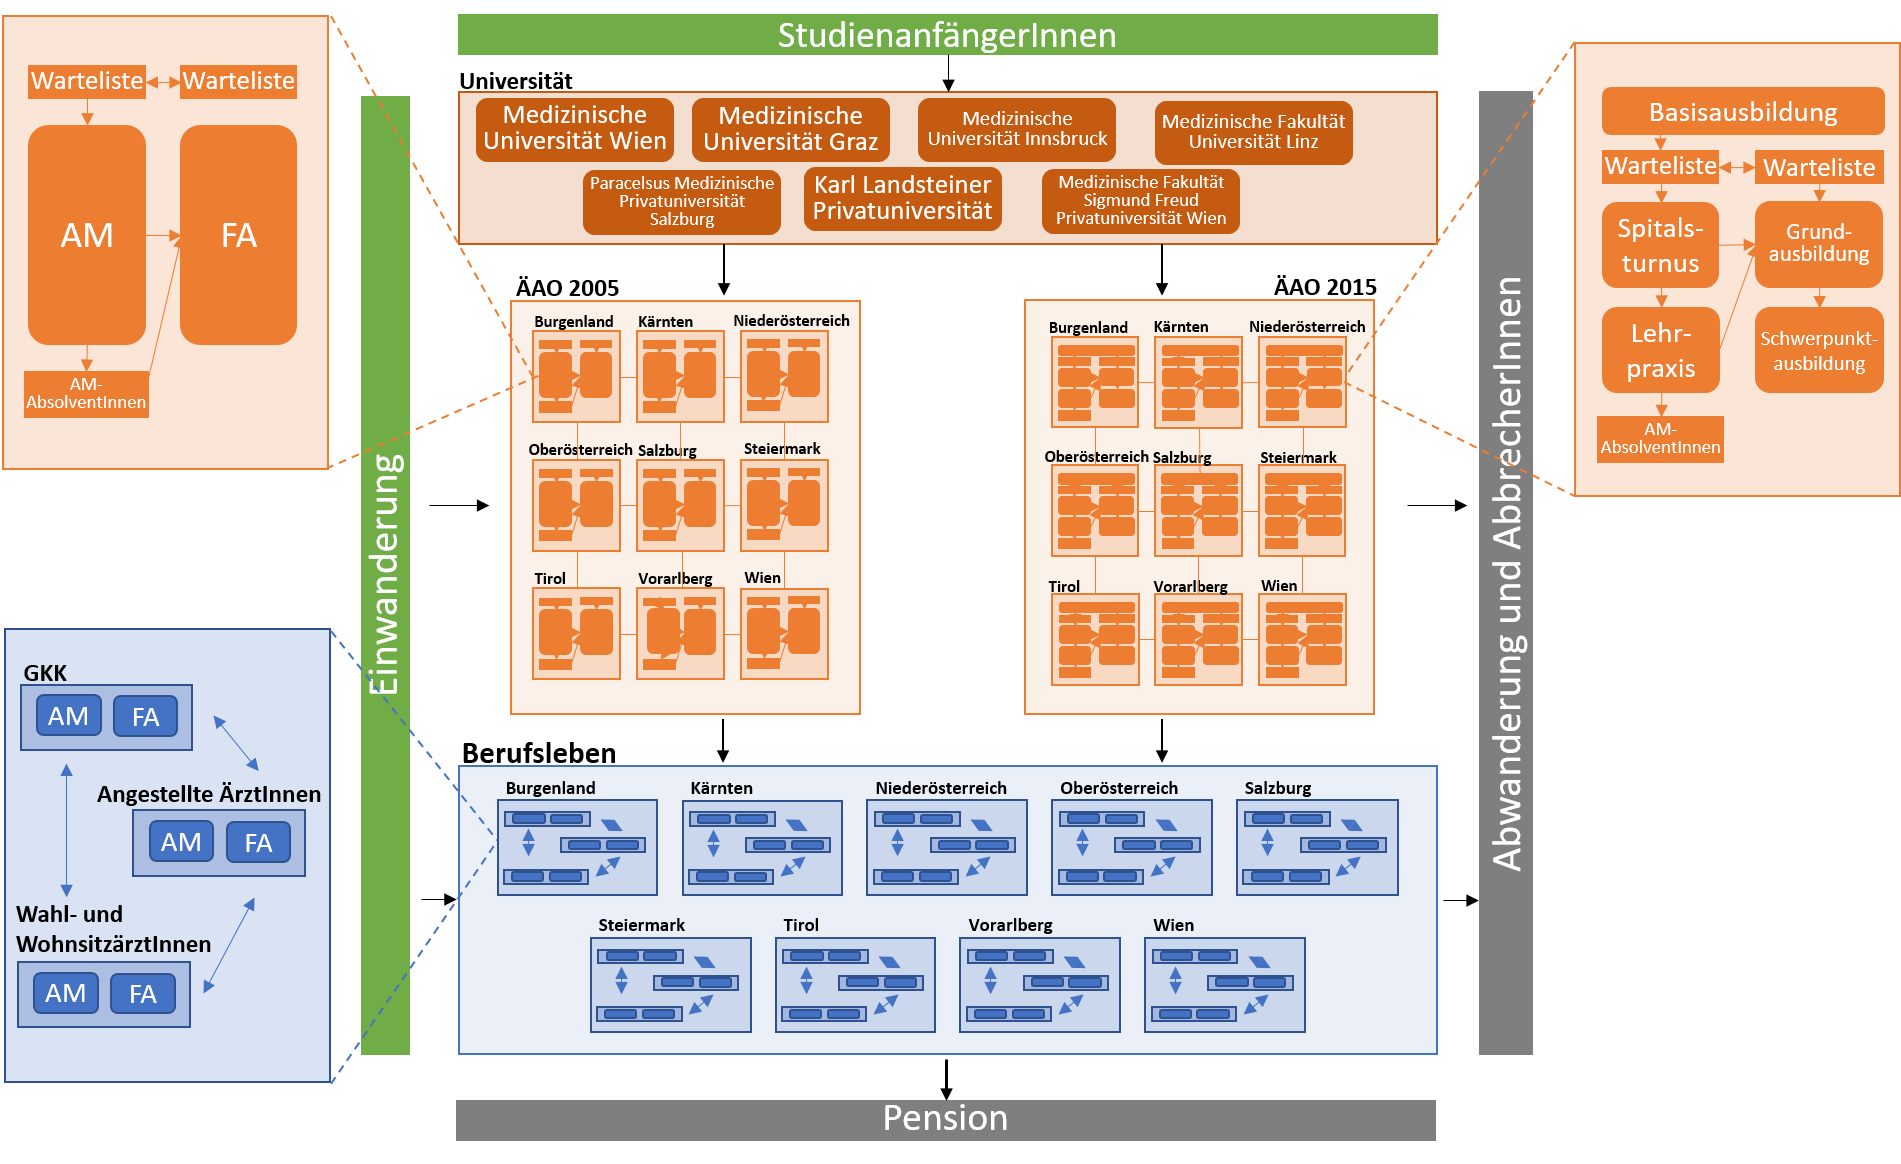
\includegraphics[width=\textwidth]{modellgraph.png}
\caption{Karrierestationen der Agenten im Modell}
\end{figure}


\subsection{Die Aufgabenstellung}

Diese Seminararbeit beschäftigt sich mit der optimalen Wahl der Anzahl der Ausbildungsstellen, jeweils für Allgemeinmediziner und Fachärzte. Jedes Jahr, wenn ÄrztInnen in Pension gehen, werden offene Stellen hinterlassen, die idealerweise durch Berufseinsteiger gefüllt werden. Ziel ist es, möglichst genau so viele Absolventen wie offene Stellen in den jeweiligen Bereichen zu haben.

\subsection{Das vereinfachte Modell}

Es wird keine Rücksicht auf das Bundesland, in dem ein angehender Arzt seine Ausbildung absolviert, sowie die Fachrichtung eines angehenden Facharztes genommen. Es werden nur die Anzahl der freien Stellen und Absolventen aller Fachrichtungen in ganz Österreich verglichen. Optional wird die Anzahl der Ausbildungsstellen für je drei Jahre zusammengefasst. Dies bewirkt eine Dimensionsreduktion im Parameterraum.

Sei also $J := \{2016,2017,\hdots,2030\}$ der Simulationszeitraum. Sei $J' := \{2019,2020,\hdots,2030\}$ der Outputzeitraum. Formal gesehen ist das Modell dann eine Funktion $\mathcal M$:

\begin{equation*}
\mathcal M: \mathbb{N}^J \times \mathbb{N}^J \rightarrow \mathbb{N}^{J'} \times \mathbb{N}^{J'} \times \mathbb{N}^{J} \times \mathbb{N}^{J}
\end{equation*}
\begin{equation*}
AM_a, FA_a \mapsto AM_f, FA_f, AM_o, FA_o
\end{equation*}

mit folgender Notation:

\begin{center}
\begin{tabular}{ | c | c | l | r |}
\hline
$AM_a$ & $FA_a$ & gesamte Ausbildungsstellen & Modellparameter \\ \hline
$AM_f$ & $FA_f$ & Berufseinsteiger (f wie fertig) & Modellresultat \\ \hline
$AM_o$ & $FA_o$ & offen gebliebene Ausbildungsstellen & Modellresultat \\ \hline
$AM_p$ & $FA_p$ & pensionierte Ärzte & vorgegebener Zielwert \\ \hline
\end{tabular}
\end{center}

$AM_p = (683, 553, 546, 519, 501, 359, 307, 291, 269, 252, 239, 211)$

$FA_p = (1082, 856, 880, 956, 978, 812, 761, 762, 752, 723, 680, 635)$

\section{Bewertungsfunktionen}

Um Optimierungsalgorithmen anwenden zu können, braucht man eine Möglichkeit, zwei Modellresultate zu vergleichen. Wir tun dies mittels einer zu minimierenden Bewertungsfunktion $\mathcal F$:

\begin{equation*}
\mathcal F: \mathbb{N}^J \times \mathbb{N}^J \times \mathbb{N}^{J'} \times \mathbb{N}^{J'} \times \mathbb{N}^{J} \times \mathbb{N}^{J} \times \mathbb{N}^{J'} \times \mathbb{N}^{J'} \rightarrow \mathbb R
\end{equation*}
\begin{equation*}
AM_a, FA_a, AM_f, FA_f, AM_o, FA_o, AM_p, FA_p \mapsto \mathcal F(\hdots)
\end{equation*}




\subsection{Die erste Bewertungsfunktion}

Die erste Bewertungsfunktion ist:

\begin{align*}
\mathcal F_1(\hdots) = c_1 &\cdot \left\| \frac{(AM_f - AM_p)}{AM_p} \cdot (1, \cdots, 0.5)  \right\|_2 + \\
			  c_2 &\cdot \left\| \frac{(FA_f - FA_p)}{FA_p} \cdot (1, \cdots, 0.5)  \right\|_2  +\\
			  c_3 &\cdot \left\| \left( \frac{ \sum\nolimits_{j=2018}^i AM_{f,j} - AM_{p,j} }{\sum\nolimits_{j=1}^i AM_{p,j} } \right)_{i\in J'} \right\|_2 +\\
			  c_4 &\cdot \left\| \left( \frac{ \sum\nolimits_{j=2018}^i FA_{f,j} - FA_{p,j} }{\sum\nolimits_{j=1}^i FA_{p,j} } \right)_{i\in J'} \right\|_2 +\\
			  c_5 &\cdot \left\| \frac{AM_o}{AM_a} \right\|_2 +\\
			  c_6 &\cdot \left\| \frac{FA_o}{FA_a} \right\|_2 
\end{align*}

wobei die Divisionen und die Multiplikationen als komponentenweise zu verstehen sind. Die ersten beiden Terme bestrafen Abweichungen zum Zielwert, also die Diskrepanz zwischen Berufseinsteigern und Pensionierten. Dies ist mit einer Diskontierung versehen, um Abweichungen in naher Zukunft stärker zu gewichten wie Abweichungen gegen Ende der untersuchten Periode. 

Die zweiten zwei Terme bestrafen kumulierten Fehler. Betrachten wir folgende Beispiele: 1) In einem Jahr gibt es 200 Anfänger zu wenig, im darauffolgenden Jahr 200 zu viel. 2) In beiden Jahren sind 200 Anfänger zu wenig. Beide Beispiele werden von den ersten beiden Termen gleich bewertet, doch in der Realität ist das erste Beispiel wünschenswerter, da die Lücken vom ersten Jahr ja im Nächsten gefüllt werden. 

Die dritten zwei Komponenten bestrafen offene Ausbildungsstellen. Dies ist offensichtlich davon motiviert, keine Ressourcen zu verschwenden.

Die Koeffizienten $\vec c$ wurden anfänglich als $(1,1,1,1,2,2)$ gewählt und dies scheint keine schlechte Wahl gewesen zu sein.

%
%\subsection{Der Zielbereich der ersten  Bewertungsfunktion}
%
%Der Fehler besteht aus 6 Summanden, die jeweils aus 12 (1-4) oder 15 (5-6) Summanden besteht. Jeder Term hier liegt zwischen und 0 und ungefähr 1. Ein Summand kann größer als 1 sein, falls zum Beispiel mehr als doppelt so viele Jungärzte fertig werden wie pensioniert werden, also sehr selten.
%
%Das Minimum der Fehlerfunktion ist also 0. Es wird erreicht, wenn alle Lücken durch Pensionierungen genau gefüllt werden und alle Ausbildungsplätze besetzt sind. Ideal, aber unrealistisch.

\subsection{Die zweite Bewertungsfunktion}

Die zweite Bewertungsfunktion ist eine Erweiterung der ersten:

\begin{align*}
\mathcal F_2(\hdots) =	\mathcal F_1&(\hdots) \hspace{4pt} + \\
			c_7 &\cdot \sum\limits_{i\in J\backslash\{2016\}} \left( \frac{AM_{a,i-1} - AM_{a,i} }{1000} \right) ^ 4 + \\
			c_8 &\cdot \sum\limits_{i\in J\backslash\{2016\}} \left( \frac{FA_{a,i-1} - FA_{a,i} }{1000} \right) ^ 4
\end{align*}

Nach ein paar Testläufen ist aufgefallen, das immer wieder Lösungen gefunden werden, in denen die Anzahl der Ausbildungsstellen stark schwingt. Dies ist natürlich unrealistisch, da zum Beispiel viele Ausbildungsplätze schaffen, nur um den Großteil davon in 3 Jahren wieder abzuschaffen ist eine Verschwendung von Ressourcen. Deshalb wurde die erste Fehlerfunktion um weitere zwei Terme erweitert, die große Sprünge bestraft. 

Der Koeffizienten $\vec c$ wurden auf $(1,1,1,1,2,2,2,2)$ erweitert. 

\subsection{Die dritte Bewertungsfunktion}

Im Laufe des Testens ist aufgefallen, dass manchmal im Laufe eines Downhill-Simplex-Algorithmus die Anzahl der Ausbildungsstellen divergieren.\footnote{Die vermeintlichen Lösungen entsprechen freiem Zugang zu Ausbildungsstellen, welcher vielleicht die beste Lösung zum Problem des Ärztemangels wäre.} Nachdem lange erfolglos ein Fehler im Algorithmus gesucht wurde, wurde klar, dass der Fehler in der Bewertungsfunktion liegt. In der fünften und sechsten Komponente steht der Anteil an unbesetzten Ausbildungsstellen. Ob dieser nun 99\% oder 99.9\% ist, macht nur ein winzigen Unterschied für die Bewertungsfunktion, aber entspricht (bei gleich vielen Auszubildenden) einer zehnfachen Erhöhung der Ausbildungsstellen. Zur Korrektur wird auf die betreffenden Terme eine Funktion angewandt, die in der Nähe der $0$ ähnlich wie die Identität ausschaut \footnote{Diese Bedingung sorgt dafür, dass $\mathcal F_2 \leq \mathcal F_3$ immer und $\mathcal F_2 \approx \mathcal F_3$ bei kleinen Anteilen der unbesetzten Ausbildungsstellen.} und bei $1$ gegen $\infty$ konvergiert.

\begin{equation*}
f: [0,1) \rightarrow [0,\infty) : x \mapsto \frac{x}{1-x}
\end{equation*}

erfüllt diese Eigenschaften und die dritte Bewertungsfunktion lautet somit:

\begin{align*}
\mathcal F_3(\hdots) = \hdots & \hspace{4pt} + \\
			c_5 &\cdot \left\| f\left( \frac{AM_o}{AM_a} \right) \right\|_2 +\\
			c_6 &\cdot \left\| f\left( \frac{FA_o}{FA_a} \right) \right\|_2 +\\
			 \hdots &
\end{align*}


\newpage

\section{Kalibrierungsansätze}

Das Problem verlangt nach Algorithmen, die nur mit Funktionsauswertungen auskommen und keine Gradienten oder Richtungsableitungen brauchen, da die Parameter des Modells ja natürliche Zahlen sind und numerische Gradientenbestimmung sowieso zu teuer wäre.

Die drei verwendeten Algorithmen haben einiges gemeinsam. Als gemeinsame Argumente haben sie eine Funktion $f: \mathbb{R}^d \rightarrow \mathbb{R}$, die Dimension $d$ und eine Matrix $bounds = \binom{a_1, \cdots, a_d}{b_1, \cdots, b_d} \in \mathbb{R}^{2\times d}$, die einen Quader $\bigtimes\nolimits_{i=1}^d [a_i, b_i] \subset \mathbb{R}^d$ beschreibt. Aus diesem Quader werden die Startwerte gewählt. Das gesuchte Minimum sollte in diesem Quader sein. 

Als Output haben die Algorithmen (natürlicherweise) den Input für die Funktion $f$ wo das Minimum vermutet ist. 

Durch die unmittelbare Anwendungsnähe ist Echtzeit-Laufzeit das wichtigste Bewertungskriterium. Durch die moderne Prozessorarchitektur mit mehreren Kernen betrachten wir auch die Parallelisierbarkeit der Algorithmen. Da die Verwendung von mehreren Kernen in einem Simulationsdurchlauf nicht einfach möglich ist, bzw. nicht im Scope dieser Seminararbeit liegt, müssen wir uns mit der parallelen Ausführung von mehreren Simulationsdurchläufen begnügen.

\subsection{Partikelschwarm \cite{kennedy_eberhart_1995}\cite{shi_eberhart_1998}}

Dieser Algorithmus basiert auf einem Schwarm von Partikeln die sich durch den Parameterraum bewegen. Zu Beginn des Algorithmus werden die Positionen von einer Anzahl an Partikeln innerhalb der $bounds$ sowie deren Geschwindigkeit zufällig gewählt. In jedem Schritt wird die Geschwindigkeitsänderung, also eine Beschleunigung ausgerechnet. Diese zieht die Partikel zum Teil zu dem bisher besten Punkt, den der jeweilige Partikel erreicht hat und zum Teil zum bisher besten Punkt überhaupt. Zur Geschwindigkeit wird dann jeweils die Beschleunigung addiert und zur Position die Geschwindigkeit. 

\begin{algorithm}[H]
\caption{Partikelschwarm}
\begin{algorithmic}
\Function{findminimum}{$f,d,bounds, numOfParticles, maxVel, acc$}

\State{$I := \{1,2,\hdots,numOfParticles\}$}

\For{$i \in I$} \Comment{für jeden Partikel}
\State{initialisiere $pos_i$ als zufällig gewählte Position innerhalb der $bounds$}
\State{initialisiere $vel_i =$ als zufällig gewählte Richtung}
\State{$pBest_i = \infty$} \Comment{der "persönlich" beste Wert}
\State{initialisiere $pBestPos_i$}
\EndFor

\State{$gBest = \infty$} \Comment{bester Wert "global"}
\State{initialisiere gBestPos}
\\
\For{$k \in \mathbb{N}_{< totalSteps}$}

	\For{$i \in I$}
	
		\If{$f(pos_i) < pBest_i$}
			\State{$pBest_i = f(pos_i)$}
			\State{$pBestPos_i = pos_i$}
			\If{$pBest_i < gBest$}
				\State $gBest = pBest_i$
				\State $gBestPos = pBest_i$
			\EndIf
		\EndIf
	
	\EndFor
	\\
	\For{$i \in I$}
		\State $vel_i = vel_i + acc \cdot rand() \cdot (pBestPos_i - pos)$
		\State $vel_i = vel_i + acc \cdot rand() \cdot (gBestPos - pos)$
		\\\Comment rand() generiert auf $[0,1]$ uniform verteile unabhängige Zufallsvariablen.
		
		\If{$||vel_i|| > maxVel$}
			\State $vel_i = maxVel \cdot \frac{vel_i}{||vel_i||}$
		\EndIf
		
		\State $pos_i = pos_i + vel_i$
	\EndFor
	
\EndFor

\Return $gBestPos$

\EndFunction
\end{algorithmic}
\end{algorithm}


%\lstinputlisting[language=python, firstline = 52 , lastline = 98]{../particleswarm.py}

\subsection{Sintflut \cite{dueck_1993} }

Der Sintflut-Algorithmus ist eine Verbesserung des naiven Hill-Climbing-Algorithmus, welcher an einem zufälligen Punkt im Parameterraum startet und dann iterativ zufällige Schritte macht. Bei einer Verbesserung wird der neue Punkt angenommen, sonst bleibt man beim alten Punkt. Eine große Schwäche des Hill-Climbing-Algorithmus ist das leichte Verfangen in lokalen Optima. Der Sintflut-Algorithmus verspricht diese Schwäche zu korrigieren.

Bildlich gesprochen befindet sich ein herumirrender Wanderer in einer Landschaft mit Hügeln und Tälern.\footnote{Für die bildliche Vorstellung suchen wir jetzt das Maximum, nicht das Minimum wie oben angegeben} Es regnet konstant und so steigt der Wasserspiegel immer weiter an. Der Wanderer, anders als im Hill-Climbing-Algorithmus kann jetzt auch bergab gehen, aber er kann nicht schwimmen. Wenn der Wanderer schließlich keinen Schritt mehr machen kann, ohne nasse Füße zu bekommen, muss er wohl einen Gipfel erreicht haben. Durch die Möglichkeit bergab zugehen erhofft man sich die gröbere Toleranz gegenüber lokalen Optima.

\begin{algorithm}
\caption{Sintflut}
\begin{algorithmic}
\Function{findminimum}{$f, d, bounds, initialLevel, deltaLevel, Schrittweite, (optional) Startparameter$}

\State initialisiere $x$ innerhalb der $bounds$

\State $level = initialLevel$

\For{$k \in \mathbb{N}_{< totalIterations}$}

	$dx \sim N(0, stepsize)$

	\If $f(x + dx) < level$
	
		\State $x = x + dx$
		\State $level = level - deltaLevel$
	\EndIf

\EndFor

\EndFunction	
\end{algorithmic}
\end{algorithm}

Die Wahl des Startwasserstands und der Regenmenge ist von großer Bedeutung. Bei zu tiefen Wasserstand wandert man unbeschränkt herum und verschwendet effektiv Rechenzeit, oder schlimmer sogar wandert weit weg vom (z.B. als gute Schätzung gewählten) Startwert. Bei zu hohem Wasserstand startet der Wanderer vielleicht schon in mitten eines Ozeans, weit weg von Land. Der Algorithmus bricht dann schnell ohne Ergebnis ab.

Die Regenmenge kontrolliert quasi die Konvergenzrate. Bei zu viel Regen kann der Wanderer vielleicht nicht schnell genug auf einen Berg flüchten. Je weniger Regen, desto länger dauert die Ausführung des Algorithmus, doch die Genauigkeit und die Konfidenz in das Ergebnis steigt.

In der originalen Quelle ist nur von einer kleinen stochastischen Änderung die Rede. Welche Verteilung diese haben soll wird nicht näher spezifiziert. Eine naheliegende Möglichkeit ist die Normalverteilung mit $\mu = 0$ und $\sigma$ als kleinen Wert der als Schrittweitenparameter betrachtet werden kann.\footnote{Der Wanderer ist dann ein Wiener.} Eine andere Möglichkeit ist eine feste Schrittweite in eine zufällige Richtung zu gehen. Letztlich wurde eine Affinkombination dieser beiden gewählt. 

%%% Normalverteilung, normierte Normalverteilung (also konstanter Schrittweite in zufällige Richtung, deren Linearkombination (also die Tischtuch über Donut-Verteilung) %%%





\subsection{Downhill Simplex \cite{nelder_mead_1965} }

Dieser Algorithmus basiert auf einem Simplex im Parameterraum, also der konvexen Hülle von $d+1$ vielen Punkten. Die Eckpunkte werden ausgewertet und in jedem Schritt wird der schlechteste Eckpunkt durch einen besseren ersetzt. Der Simplex bewegt sich dadurch im Laufe der Zeit dem figurativen Hügel hinab einem lokalen Minimum entgegen und zieht sich letztendlich über dem Minimum zusammen.

\begin{algorithm}
\caption{Downhill Simplex}
\begin{algorithmic}
\Function{findminimum}{$f, d, bounds, \alpha = 1, \gamma = 2, \beta = \frac{1}{2}, \sigma = \frac{1}{2}$}

\State $x_i$ für $i \in \mathbb{N}_{\leq d}$ werden zufällig innerhalb der $bounds$ gewählt

\For{$k \in \mathbb{N}_{< totalSteps}$}

\State sortiere $x_i$ sodass $f(x_0) < f(x_1) < \hdots < f(x_d)$

\State $m := \frac{1}{d} \sum^{d-1}_{i = 0} x_i$ \Comment{der Mittelpunkt aller Ecken außer der schlechtesten}

\State $r := (1+\alpha)m - \alpha x_d$ \Comment{Der Reflektierte Punkt}

\If{$f(r) < f(x_0)$}

\State $e := (1+\gamma)m - \gamma x_d$ \Comment{Der Expandierte Punkt}

\If{$f(e) < f(r)$}
\State $x_d := e$
\Else
\State $x_d := r$
\EndIf

\ElsIf{$f(r) < f(x_{d-1})$}
\State $x_d := r$
\Else

\If{$f(r) < f(x_N)$}
\State $h := r$

\Else
\State $h := x_d$

\EndIf

\State $c := \beta m  + (1-\beta) h$

\If{$f(c) < f(x_d)$} 

\State $x_d := c$ \Comment{Der Kontrahierte Punkt}

\Else

\State $x_i := \sigma x_0 + (1-\sigma) x_i \forall i \neq 0$ \Comment{Komprimiere den Simplex}

\EndIf

\EndIf

\EndFor

\Return $x_0$
\EndFunction	
\end{algorithmic}
\end{algorithm}

\begin{figure}[h]
\includegraphics[width=\textwidth]{downhillsimplex_big.png}
\caption{Simplex in der Ebene, sowie die vier neuen Möglichkeiten für $x_3$}
\end{figure}

Im Pseudocode wurde $f$ hier oftmals zur Klarheit doppelt und dreifach aufgerufen. In der tatsächlichen Implementation wird $f$ für jeden Punkt natürlich nur einmal aufgerufen und das Ergebnis gespeichert.


\subsection{Vergleich}

Die drei Ansätze profitieren unterschiedlich von der Verfügbarkeit von vielen Prozessorkernen. 

Der Partikelschwarm-Algorithmus eignet sich hervorragend zu Parallelisierung. Die Partikel bewegen sich alle gemeinsam in einem Zeitschritt und deren neue Position muss danach gleichzeitig ausgewertet werden. Idealerweise wählt man dann auch noch die Anzahl der Partikel als ein Vielfaches der Anzahl der verfügbaren Prozessorkerne um alle Kerne immer zu nutzen. Bei vielen Kernen kann man die Anzahl der Partikel einfach der Anzahl der Kerne gleichsetzen. So verwendet man nahezu 100\% der verfügbaren Rechenleistung und verwendet außerdem alle ausgewerteten Stellen sinnvoll im weiteren Verlauf.

Der Sintflut-Algorithmus profitiert hingegen sehr wenig von Parallelisierung. Man kann spekulativ mehrere mögliche Schritte zugleich auswerten und falls der erste ins Wasser steigt, den zweiten überprüfen und so weiter. Man erkauft sich dadurch ein bisschen Beschleunigung, aber viele der Auswertungen fließen gar nicht in den Algorithmus ein. Mit steigender Prozessorkernanzahl trifft man schnell auf $diminishing$ $returns$.

Für den Downhill Simplex-Algorithmus gibt es in jedem Schritt zwei Möglichkeiten, entweder der schlechteste Punkt $x_d$ wird ersetzt oder der Simplex wird komprimiert.

Im ersten Fall gibt es vier Kandidaten für die neue Stelle des Eckpunkts, nämlich $r$, $e$ und zwei mal $c$, je nachdem ob $h$ als $r$ oder $x_d$ gewählt wird. Diese vier Möglichkeiten können gleichzeitig ausgewertet werden und man erkauft sich eine bis zu dreifache Beschleunigung. 

Beim ersten Auswerten der Eckpunkte zu Beginn und beim Kontrahieren des Simplex kann natürlich auch parallelisiert werden.

%TODO: spekulativ 2 Schritte, kerne $>$ d
%
%\begin{center}
%\begin{tabular}{| l | r | r | r |}
%\hline
%				& Partikelschwarm & Sintflut & Downhill Simplex \\ \hline
%Gewinn durch mehr Prozessorkerne & Gut& Meh & Mäßig \\ \hline
%Sinnhaftigkeit einer Tabelle hier & Mäßig & Hmm & Nicht so \\ \hline
%&&& \\ \hline
%\end{tabular}
%\end{center}


\section{Technische Details}

Die gesamte Codebase ist in Python 3 geschrieben. Das Modell ist als importierte Funktion aufrufbar. Da die Signatur dieser Funktion ein $dict$ ist, welches Einträge für je Allgemeinmediziner und Fachärzte hat, die Algorithmen aber ein einzelnes $numpy$-Array erwarten wurde ein Wrapper für das Modell implementiert, der Argumente übersetzt. Dieser wendet auch gleich die Bewertungsfunktion auf das Modellresultat an. Auf diese Weise können die Algorithmen komplett modellagnostisch implementiert werden. 

Zusätzlich schreibt der Wrapper alle Funktionsaufrufe einer Ausführung in einer $.csv$ Datei mit. Es werden die Parameter, die Modellergebnisse, der Wert der Bewertungsfunktion sowie die einzelnen Komponenten der Bewertungsfunktion gespeichert. Diese Logs ermöglicht detaillierte Analyse des Konvergenzverhaltens.

\section{Resultate}

\subsection{Experiment 1}

Wir führen die drei Algorithmen mehrmals durch und beobachten Konvergenzverhalten und erzielte Werte. Die Parameter werden für je 3 Jahre konstant gehalten. Damit ist die Dimension $d = 10$. Die Startwerte werden aus $bounds = [0,1500]^d$ gewählt. Wir erlauben 160 bzw. 480 Auswertungen. Dies entspricht etwa 2 bzw. 6 Stunden Rechenzeit auf meinem 8-kernigen Prozessor.

Um das Konvergenzverhalten zu beobachten betrachten wir die Spalte für die Bewertungsfunktion in den Logs. Sei $e_i$ die Bewertung der $i$-ten Modellauswertung, also der $i$-ten Zeile im Log. Wir betrachten $m_i := min\left\{e_k:k\leq i\right\}$. Dies ist die Bewertung, wenn man den Algorithmus nach $i$ Modellauswertungen abbrechen würde. Die Folge der $m_i$ ist durch Definition monoton fallend und flacht ab wenn ein (zumindest lokales) Minimum gefunden wird. 

\begin{figure}[h]
\includegraphics[width = \textwidth/2]{5p_neu_convergence_plot_Partikelschwarm.png}
\includegraphics[width = \textwidth/2]{5p_neu_convergence_boxplot_Partikelschwarm.png}
\caption{Konvergenzrate: Partikelschwarm}
\end{figure}

Beim Partikelschwarm sieht man, dass stetige Verbesserungen auch noch spät gefunden werden. Man kann vermuten, dass mehr Auswertungen durchaus zu mehr besseren Ergebnissen führen würden. Nur 160 Auswertungen sind definitiv zu wenig für den Partikelschwarm. 

\begin{figure}[h]
\includegraphics[width = \textwidth/2]{5p_neu_convergence_plot_Sintflut.png}
\includegraphics[width = \textwidth/2]{5p_neu_convergence_boxplot_Sintflut.png}
\caption{Konvergenzrate: Sintflut}
\end{figure}

Die Bewertungen beim Sintflut-Algorithmus sind kreuz und quer. Manche passen gar nicht auf die Skala während ein anderer Durchgang nach nur 11 Auswertungen einen der besten Werte insgesamt findet, oder besser gesagt, errät. Diese große Varianz macht den Algorithmus unbrauchbar.

\begin{figure}[h]
\includegraphics[width = \textwidth/2]{5p_neu_convergence_plot_Downhill_Simplex.png}
\includegraphics[width = \textwidth/2]{5p_neu_convergence_boxplot_Downhill_Simplex.png}
\caption{Konvergenzrate: Downhill Simplex}
\end{figure}

Der Downhill Simplex-Algorithmus konvergiert sehr schnell innerhalb der ersten 160 Auswertungen und bleibt dann in einem lokalen Minimum liegen. Er profitiert nicht wirklich von mehr Auswertungen. Die schnelle und sehr konsistene Konvergenzrate ist ein Vorteil.

%\subsubsection{Vergleich}
%\includegraphics{5p_neu_convergence_plot_alle_gemeinsam.png}
\begin{center}
\begin{tabular}{| l || r | r | r || r | r | r ||}
\hline
        & \multicolumn{3}{l||}{160 Auswertungen} & \multicolumn{3}{l||}{480 Auswertungen} \\ \hline
        & Partikel &          & Downhill & Partikel &          & Downhill\\ 
        & schwarm  & Sintflut & Simplex  & schwarm  & Sintflut & Simplex\\ \hline
Anzahl der Durchführungen  & 24 & 24 & 24 & 14 & 14 & 13 \\ \hline
Mittelwert                 & 3.94 & 6.99 & 4.50 & 3.25 & 6.95 & 4.39 \\ \hline
Median                     & 3.95 & 7.07 & 4.39 & 3.14 & 7.34 & 4.42 \\ \hline
Varianz                    & 0.53 & 4.59 & 0.96 & 0.34 & 5.16 & 1.12 \\ \hline
Bester Wert                & 2.73 & 2.58 & 2.55 & 2.53 & 2.58 & 2.49 \\ \hline
Schlechtester Wert         & 5.91 &11.39 & 6.56 & 4.24 &10.04 & 5.89 \\ \hline
Durchschnitt der TOP3      & 2.84 & 3.18 & 2.90 & 2.55 & 3.76 & 2.82 \\ \hline
\end{tabular}
\end{center}

\subsection{Experiment 2}

Für das zweite Experiment geben wir keine Einschränkungen an die Parameter vor. Jedes Jahr ist unabhängig von den anderen. Damit ist $d = 30$. Wie zuvor seinen die $bounds = [0,1500]^d$. Die Anzahl der erlaubten Auswertungen wird auf 2400 erhöht.

\begin{figure}[h]
\includegraphics[width = \textwidth/2]{15p_convergence_plot_Partikelschwarm.png}
\includegraphics[width = \textwidth/2]{15p_convergence_boxplot_Partikelschwarm.png}
\caption{Konvergenzrate: Partikelschwarm}
\end{figure}

\begin{figure}[h]
\includegraphics[width = \textwidth/2]{15p_convergence_plot_Sintflut.png}
\includegraphics[width = \textwidth/2]{15p_convergence_boxplot_Sintflut.png}
\caption{Konvergenzrate: Sintflut}
\end{figure}

\begin{figure}[h]
\includegraphics[width = \textwidth/2]{15p_convergence_plot_Downhill_Simplex.png}
\includegraphics[width = \textwidth/2]{15p_convergence_boxplot_Downhill_Simplex.png}
\caption{Konvergenzrate: Downhill Simplex}
\end{figure}


Durch die größere Freiheit in den Parametern erhofft man sich besser bewertete Lösungen, da ja der alte Parameterraum Teilmenge des neuen ist. Alle drei Algorithmen können aber leider mit der zusätzlichen Komplexität nicht umgehen und erbringen trotz verfünffachter Zeit schlechtere Bewertungen. Der Sintflut-Algorithmus leidet ganz besonders, man beachte die veränderte y-Achse.

\begin{center}
\begin{tabular}{| l || r | r | r || r | r | r ||}
\hline
        & \multicolumn{3}{l||}{1200 Auswertungen} & \multicolumn{3}{l||}{2400 Auswertungen} \\ \hline
        & Partikel &          & Downhill & Partikel &          & Downhill\\ 
        & schwarm  & Sintflut & Simplex  & schwarm  & Sintflut & Simplex\\ \hline
Anzahl der Durchführungen  & 9 & 9 & 8 & 7 & 8 & 7 \\ \hline
Mittelwert                 & 4.37 & 14.76 & 5.13 & 4.42 & 13.89 & 4.99 \\ \hline
Median                     & 4.52 & 15.26 & 4.97 & 4.33 & 13.99 & 4.94 \\ \hline
Varianz                    & 0.77 & 20.41 & 0.51 & 0.71 & 18.29 & 0.48 \\ \hline
Bester Wert                & 3.01 &  7.74 & 4.20 & 3.01 &  7.74 & 4.17 \\ \hline
Schlechtester Wert         & 5.92 & 21.74 & 6.46 & 5.92 & 21.74 & 6.46 \\ \hline
Durchschnitt der TOP3      & 3.32 &  9.43 & 4.48 & 3.70 &  9.35 & 4.45 \\ \hline
\end{tabular}
\end{center}

\subsection{Fazit}

Was ist nun der beste Kalibrierungsansatz? Die Antwort hängt vom Kontext der Kalibrierung ab. Wenn es schnell gehen soll, also in der Größenordnung von ein paar Stunden, besticht der Downhill Simplex mit seiner schnellen Konvergenzrate. Hat man mehr Zeit und wünscht sich eine bessere Güte des Ergebnisses, wird der Partikelschwarm attraktiver. Ab einer gewissen Grenze lohnt es sich aber, mehrere kürzere $Runs$ zu starten und den besten dieser zu wählen.

Kalibriert man nicht auf einem Desktop oder Laptop, sondern einem Cluster mit sehr vielen Prozessorkernen ist der Partikelschwarm definitiv der beste Ansatz aufgrund seiner überragenden Skalierbarkeit.

Die Zusammenfassung von je drei Jahren zu einem Parameter ist eine sehr sinnvolle Einschränkung. Der vermeintliche Mehrgewinn durch die Freiheit der Parameter ist die zusätzliche Komplexität nicht wert.

\section{Die besten Lösungen}

Zurück zur ursprünglichen Frage. Wie sollen die Ausbildungsstellen gewählt werden? Wir sehen uns die besten Resultate jeder Kalibrierungsmethode an. (Detailliertere Darstellungen in Appendix A)


\begin{center}
\begin{tabular}{| l | l | r | r | r | r | r |}
\hline
& & 2016-18 & 2019-21 & 2022-24 & 2025-27 & 2028-2030 \\ \hhline{|=|=|=|=|=|=|=|}
Partikelschwarm  & $AM_a$ & 271 & 718 & 366 & 304 & 376\\ \hline
				 & $FA_a$ & 680 & 909 & 676 & 547 & 401\\ \hhline{|=|=|=|=|=|=|=|}
Sintflut	     & $AM_a$ & 347 & 578 & 508 & 355 & 276\\ \hline
				 & $FA_a$ & 709 & 809 & 624 & 794 & 1089\\ \hhline{|=|=|=|=|=|=|=|}
Downhill Simplex & $AM_a$ & 338 & 621 & 455 & 371 & 532\\ \hline
				 & $FA_a$ & 602 & 907 & 956 & 874 & 832\\ \hline
\end{tabular}
\end{center}

Die Parameter sind sich in den frühen Jahren halbwegs einig, doch in den späteren Jahren klaffen sie weit auseinander. Abbildung \ref{fig:scatter} zeigt diesen Trend auch auf dem gesamten Datenset aller 25521 Auswertungen. Die 10 Subplots entsprechen den 10 Parametern und zeigen die Bewertung gegenüber der dem Parameterwert. Man erkennt dreieckige Punktwolken, deren Spitzen auf den optimalen Parameterwert zeigen. Die Parameter für Allgemeinmediziner sowie tendenziell die früheren Parameter weisen spitzere Spitzen auf. Dies deutet darauf hin, dass die sorgfältige Wahl dieser wichtiger ist als die restlichen Parameter oder zumindest, dass die Spanne von akzeptablen Werten bei kleiner ist. Bei dem Facharztparameter für 2028-30 ist gar keine Spitze zu sehen, sondern eher eine flache Front. Während dieser Parameter sicher einen Einfluss auf das Modell hat, hat er keinen oder höchstens einen winzig kleinen Einfluss auf die Bewertung. Ergo, man kann mit den hier beschriebenen Methoden keine Policy-Empfehlung für die letzten Jahre abgeben.

Die letztendliche Empfehlung lautet daher:

\begin{center}
\begin{tabular}{| l | r | r | r | r | r |}
\hline
& 2016-18 & 2019-21 & 2022-24 & 2025-27 & 2028-2030 \\ \hline
$AM_a$ & 300 & 650 & 400 & 350 & 400 \\ \hline
$FA_a$ & 750 & 900 & 800 & 700 &  ?? \\ \hline
\end{tabular}
\end{center}

Man sollte auf jeden Fall vor 2028 neu simulieren und optimieren, und gegebenenfalls schon früher.

\begin{figure}[H]
\includegraphics[width = \textwidth]{megascatterplot.png}
\caption{Scatterplot der Parameter gegenüber der Bewertung. Rot = Partikelschwarm, Grün = Sintflut, Blau = Downhill Simplex}
\label{fig:scatter}
\end{figure}

\newpage

\bibliography{bib}
\bibliographystyle{alpha}

\appendix

\section{Aufschlüsselungen}

\begin{figure}[h]
\includegraphics[width = \textwidth]{resultPlots/Partikelschwarm27.png}
\caption{Resultataufschlüsselung: bester Partikelswarm}
\end{figure}

\begin{figure}[h]
\includegraphics[width = \textwidth]{resultPlots/Sintflut27.png}
\caption{Resultataufschlüsselung: bester Sintflut}
\end{figure}

\begin{figure}[h]
\includegraphics[width = \textwidth]{resultPlots/Downhill_Simplex21.png}
\caption{Resultataufschlüsselung: bester Downhill Simplex}
\end{figure}


\begin{figure}[h]
\includegraphics[width = \textwidth]{resultPlots/Partikelschwarm5.png}
\caption{Resultataufschlüsselung: zufällig gewählter Partikelswarm}
\end{figure}

\begin{figure}[h]
\includegraphics[width = \textwidth]{resultPlots/Sintflut5.png}
\caption{Resultataufschlüsselung: zufällig gewählter Sintflut}
\end{figure}

\begin{figure}[h]
\includegraphics[width = \textwidth]{resultPlots/Downhill_Simplex5.png}
\caption{Resultataufschlüsselung: zufällig gewählter Downhill Simplex}
\end{figure}

\end{document}
































